\documentclass[11pt]{article}
\usepackage[a4paper,margin=28mm]{geometry}
\usepackage{amsmath,amssymb,amsthm}
\usepackage{tikz}
\usepackage[colorlinks=true,allcolors=blue]{hyperref}
\newtheorem{theorem}{Theorem}[section]
\newtheorem{lemma}[theorem]{Lemma}
\newtheorem{proposition}[theorem]{Proposition}
\theoremstyle{remark}
\newtheorem{example}[theorem]{Example}
\newtheorem{remark}[theorem]{Remark}

% Planar-tree glyphs; the main paper defines these in table_trees.tex.
\tikzset{tv/.style={circle,fill,inner sep=0pt,minimum size=2.4pt},
  tree/.style={baseline=(r.south),x=0.8ex,y=0.8ex}}
\providecommand{\TLeaf}{\tikz[tree]\node[tv](r){};}
\providecommand{\TChainTwo}{\tikz[tree]{\node[tv](r)at(0,0){};\node[tv](b)at(0,1.5){};\draw(r)--(b);}}
\providecommand{\TChainThree}{\tikz[tree]{\node[tv](r)at(0,0){};\node[tv](b)at(0,1.5){};\node[tv](c)at(0,3){};\draw(r)--(b)--(c);}}
\providecommand{\TTwoLeaves}{\tikz[tree]{\node[tv](r)at(0,0){};\node[tv](b)at(-0.8,1.5){};\node[tv](c)at(0.8,1.5){};\draw(b)--(r)--(c);}}

\newcommand{\one}{\mathbf 1}
\newcommand{\bA}{\mathbf A}
\newcommand{\bb}{\mathbf b}
\newcommand{\bc}{\mathbf c}
\newcommand{\ba}{\mathbf a}
\newcommand{\bw}{\mathbf w}
\newcommand{\bbeta}{\boldsymbol\beta}
\newcommand{\bPhi}{\boldsymbol\Phi}
\newcommand{\bg}{\mathbf g}
\newcommand{\Area}{\operatorname{Area}}
\newcommand{\Tpl}{\mathcal T^{\mathrm{pl}}}
\newcommand{\Fpl}{\mathcal F^{\mathrm{pl}}}
\newcommand{\phiex}{\phi_{\mathrm{ex}}}

\begin{document}

% Labels defined in ees_simods.tex; delete this block when merging.
\newcounter{ext}\renewcommand{\theext}{M\arabic{ext}}
\newcommand{\extlabel}[1]{\refstepcounter{ext}\label{#1}}
\extlabel{eq:2n_rk}\extlabel{eq:bazavov-cf-lift}\extlabel{eq:cfees25-betas-general}%
\extlabel{eq:williamson-unroll}\extlabel{eq:owren-exponential}\extlabel{eq:cfees-row-recursion}%
\extlabel{eq:cfees-pseudostage}\extlabel{thm:cosine-ees-order}\extlabel{thm:cfees-order-main}%
\extlabel{prop:frozen-expansion}\extlabel{eq:forest-order-two}\extlabel{eq:cosine25-tables}%
\extlabel{tab:alpha-cf-ees25-x}%

\section{Forward order for general Williamson coefficients}
\label{sec:order-transfer}

We show that the commutator-free method \eqref{eq:bazavov-cf-lift} inherits the classical order of the Runge--Kutta method \eqref{eq:2n_rk}, for arbitrary real coefficients $(A_i,B_i)_{i=1}^s$ and every order $p$. Two facts drive the proof. First, the piecewise-linear path through the rows of $\bA$ and then $\bb^\top$, with one segment for each exponential, has a signature whose coefficients are exactly the order conditions of the commutator-free method. Second, for Williamson coefficients the signed area between two linear projections of this path is again a linear projection. Since iterated areas generate the shuffle algebra \cite{diehl2020areas}, every coefficient of the lifted method is a universal polynomial in the classical elementary weights. The exact flow has the same structure, so the lifted coefficients agree with those of the exact flow whenever the elementary weights do.

\subsection{The coefficient path}

Let $\bbeta_i=(\beta_{i1},\ldots,\beta_{is})$ be the $i$th row of the coefficients \eqref{eq:cfees25-betas-general}, with $\beta_{ij}=0$ for $j>i$. Equivalently, $\bbeta_i=B_i\bw_i$, where
\begin{equation}
\label{eq:williamson-rows}
\bw_0=0,\qquad \bw_i=A_i\bw_{i-1}+\mathbf e_i^\top,
\end{equation}
and $\mathbf e_i^\top$ is the $i$th coordinate row. By \eqref{eq:williamson-unroll}, the rows $\ba_i$ of the Butcher matrix $\bA=(a_{ij})$ and the weights $\bb$ are partial sums of these rows. Setting $\ba_{s+1}=\bb^\top$, we have
\begin{equation}
\label{eq:tableau-rows}
\ba_i=\sum_{l<i}\bbeta_l,\qquad 1\leq i\leq s+1.
\end{equation}

The \emph{coefficient path} $x:[0,s]\to\mathbb R^{1\times s}$ is the piecewise-linear path with vertices $x(l)=\ba_{l+1}$, $0\leq l\leq s$. Its $l$th segment has increment $\bbeta_l$. For $u\in\mathbb R^s$, write $x^u=xu$ for the scalar projection, and for $u_1,\ldots,u_m\in\mathbb R^s$ write
\[
S_t(u_1\cdots u_m)=\int_{0<t_1<\cdots<t_m<t}\mathrm dx^{u_1}_{t_1}\cdots\mathrm dx^{u_m}_{t_m},
\qquad S_t(\emptyset)=1,
\]
for the signature of $x$ paired with $u_1\otimes\cdots\otimes u_m$. Along the $l$th segment each $x^{u_r}$ grows linearly, by $\bbeta_lu_r$, and the iterated integral over that segment alone is $\frac1{m!}\prod_r\bbeta_lu_r$. Integrals over several segments are built from these by Chen's identity, which sorts the ordered times $t_1<\cdots<t_m$ into the segments they fall in.

\begin{example}
\label{ex:path-williamson}
Williamson's three-stage scheme of classical order three has coefficients $A_i=0,-\frac59,-\frac{153}{128}$ and $B_i=\frac13,\frac{15}{16},\frac8{15}$, so $\bbeta_1=(\frac13,0,0)$, $\bbeta_2=(-\frac{25}{48},\frac{15}{16},0)$ and $\bbeta_3=(\frac{17}{48},-\frac{51}{80},\frac8{15})$. The tableau and coefficient path are
\begin{center}
\begin{minipage}[c]{0.34\linewidth}
\[
\renewcommand{\arraystretch}{1.2}
\begin{array}{c|ccc}
0&0&0&0\\
\tfrac13&\tfrac13&0&0\\
\tfrac34&-\tfrac3{16}&\tfrac{15}{16}&0\\\hline
&\tfrac16&\tfrac3{10}&\tfrac8{15}
\end{array}
\]
\end{minipage}\hfill
\begin{minipage}[c]{0.64\linewidth}
\centering
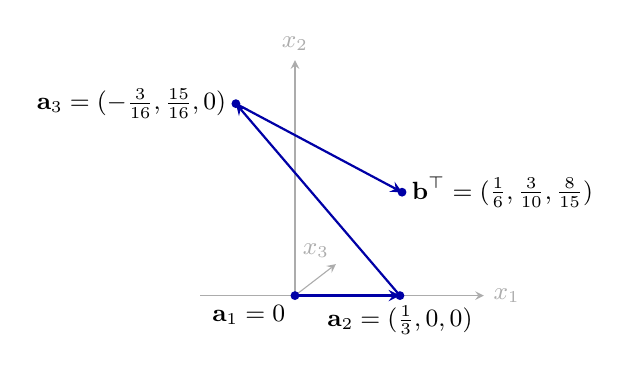
\begin{tikzpicture}[x={(4cm,0cm)},y={(0cm,2.6cm)},z={(1.3cm,1.0cm)},font=\small,>=stealth]
\coordinate (a1) at (0,0,0);
\coordinate (a2) at (1/3,0,0);
\coordinate (a3) at (-3/16,15/16,0);
\coordinate (b) at (1/6,3/10,8/15);
\draw[->,gray!65] (-0.3,0,0)--(0.6,0,0) node[right] {$x_1$};
\draw[->,gray!65] (a1)--(0,1.15,0) node[above] {$x_2$};
\draw[->,gray!65] (a1)--(0,0,0.4) node[above left=-1pt] {$x_3$};
\draw[->,thick,blue!65!black] (a1)--(a2);
\draw[->,thick,blue!65!black] (a2)--(a3);
\draw[->,thick,blue!65!black] (a3)--(b);
\foreach \p in {a1,a2,a3,b} \fill[blue!65!black] (\p) circle (1.6pt);
\node[below left] at (a1) {$\ba_1=0$};
\node[below] at (a2) {$\ba_2=(\tfrac13,0,0)$};
\node[left] at (a3) {$\ba_3=(-\tfrac3{16},\tfrac{15}{16},0)$};
\node[right] at (b) {$\bb^\top=(\tfrac16,\tfrac3{10},\tfrac8{15})$};
\end{tikzpicture}
\end{minipage}
\end{center}
\end{example}

Recall that $g_{l+1}(B_+(\tau_1\cdots\tau_k))$ is the Lie--Butcher coefficient of the forest $\tau_1\cdots\tau_k$ in the stage $Y_l$, reached after $l$ exponentials. For $l=s$ it is $\phi(\tau_1\cdots\tau_k)$, the coefficient in the MKW order condition for that forest. For a tree $\tau$, let $\bg(\tau)=(g_1(\tau),\ldots,g_s(\tau))^\top$ be its coefficients in the $s$ slopes.

By \eqref{eq:owren-exponential}, the $l$th exponential contains $\tau$ with coefficient $\mathcal V_l(\tau)=\bbeta_l\bg(\tau)$, which is how much $x^{\bg(\tau)}$ grows on the $l$th segment. Each exponential therefore acts as one straight segment of the path, and composing exponentials corresponds to appending segments.

\begin{lemma}[Lie--Butcher coefficients as signatures]
\label{lem:stages-signature}
For $0\leq l\leq s$ and $\tau_1,\ldots,\tau_k\in\Tpl$,
\[
g_{l+1}(B_+(\tau_1\cdots\tau_k))=S_l\bigl(\bg(\tau_1)\cdots\bg(\tau_k)\bigr).
\]
In particular, $\phi(\tau_1\cdots\tau_k)=S_s(\bg(\tau_1)\cdots\bg(\tau_k))$.
\end{lemma}

\begin{proof}
The increment of $x^{\bg(\tau)}$ over the $l$th segment is $\bbeta_l\bg(\tau)=\mathcal V_l(\tau)$. Hence \eqref{eq:owren-exponential} is the signature of the $l$th segment, and \eqref{eq:cfees-row-recursion} is Chen's identity for appending it. Both sides equal $\varepsilon(\tau_1\cdots\tau_k)$ when $l=0$.
\end{proof}

% Example: order conditions as areas. Input from the main section after Lemma 1.2.
\begin{example}
\label{ex:areas-williamson}
In Example~\ref{ex:path-williamson}, the nodes are $\bc=(0,\frac13,\frac34)$. By Lemma~\ref{lem:stages-signature}, the order conditions for $\TChainTwo\,\TLeaf$ and $\TLeaf\,\TChainTwo$ are $S_3(\bc\,\one)=\int x^{\bc}\,\mathrm dx^{\one}=\frac16$ and $S_3(\one\,\bc)=\int x^{\one}\,\mathrm dx^{\bc}=\frac13$: the areas below and to the left of the path in the $(x^{\one},x^{\bc})$-plane.
\definecolor{sigblue}{RGB}{70,120,200}%
\definecolor{sigorange}{RGB}{230,150,60}%
\newcommand{\sigpanel}[3]{%
\begin{tikzpicture}[x=4cm,y=4cm,font=\small,>=stealth]
\fill[sigorange,opacity=0.35] #1;
\fill[sigblue,opacity=0.45] #2;
\draw[->,gray] (0,0)--(1.12,0) node[right]{$x^{\one}$};
\draw[->,gray] (0,0)--(0,0.62) node[above]{$x^{\bc}$};
\draw[gray,dashed] (1,0)--(1,0.5)--(0,0.5);
\node[below] at (1,0) {$1$};
\node[left] at (0,0.5) {$\tfrac12$};
\node at (0.3,0.3) {$\TLeaf\,\TChainTwo\colon\tfrac13$};
\node at (0.8,0.1) {$\TChainTwo\,\TLeaf\colon\tfrac16$};
\node[above] at (0.56,0.66) {#3};
}%
\begin{center}
\sigpanel{(0,0)--(1/3,0)--(3/4,5/16)--(1,0.5)--(0,0.5)--cycle}{(1/3,0)--(3/4,5/16)--(1,0.5)--(1,0)--cycle}{Williamson}
\draw[very thick,blue!50!black] (0,0)--(1/3,0)--(3/4,5/16)--(1,0.5);
\foreach \p in {(0,0),(1/3,0),(3/4,5/16),(1,0.5)} \fill[blue!50!black] \p circle (1.3pt);
\end{tikzpicture}\hspace{0.6cm}%
\sigpanel{plot[domain=0:1,samples=60] (\x,{\x*\x/2}) -- (0,0.5) -- cycle}{plot[domain=0:1,samples=60] (\x,{\x*\x/2}) -- (1,0) -- cycle}{exact flow}
\draw[very thick,black,domain=0:1,samples=60] plot (\x,{\x*\x/2});
\end{tikzpicture}
\end{center}
The paths differ, but the areas agree, as Theorem~\ref{thm:transfer} predicts.
\end{example}


The simplest cases show what the lemma produces. With a single tree the integral is just the total growth of the path, so $\bg(B_+(\tau))=\bA\bg(\tau)$; for $\tau=\TLeaf$ this gives the vector of nodes, $\bg(\TChainTwo)=\bc=\bA\one$. With the same tree repeated, the integral is a power divided by a factorial; for example, $\bg(\TTwoLeaves)=\frac12\bc\odot\bc$. The order of the exponentials matters only when different trees appear, since in general $S_l(\bc\,\one)\neq S_l(\one\,\bc)$. Lemma~\ref{lem:area} below is what controls these terms.

\subsection{Areas are path coordinates}

Let $\mathcal T$ be the set of (non-planar) rooted trees, with $\tau!=|\tau|\,\tau_1!\cdots\tau_k!$ for $\tau=B_+(\tau_1\cdots\tau_k)$ and $\TLeaf!=1$. The elementary weight vectors $\bPhi(\tau)\in\mathbb R^s$ are
\[
\bPhi(\TLeaf)=\one,\qquad \bPhi(B_+(\tau_1\cdots\tau_k))=\bA\bPhi(\tau_1)\odot\cdots\odot\bA\bPhi(\tau_k),
\]
where $\odot$ is the componentwise product, and \eqref{eq:2n_rk} has classical order $p$ if and only if $\bb^\top\bPhi(\tau)=1/\tau!$ for all $\tau\in\mathcal T$ with $|\tau|\leq p$. For $u,v\in\mathbb R^s$ define
\[
u\triangleright v=(\bA u)\odot v,\qquad D(u,v)=u\triangleright v-v\triangleright u.
\]
If $\sigma\curvearrowright\tau=B_+(\tau_1\cdots\tau_k\sigma)$ denotes grafting $\sigma$ onto the root of $\tau=B_+(\tau_1\cdots\tau_k)$, the definition of $\bPhi$ gives $\bPhi(\sigma)\triangleright\bPhi(\tau)=\bPhi(\sigma\curvearrowright\tau)$. Extending $\bPhi$ linearly,
\begin{equation}
\label{eq:grafting}
D(\bPhi(\sigma),\bPhi(\tau))=\bPhi(\sigma\curvearrowright\tau-\tau\curvearrowright\sigma).
\end{equation}
For scalar paths $f,g$ with $f(0)=g(0)=0$, write $\Area(f,g)_t=\int_0^tf\,\mathrm dg-g\,\mathrm df$, twice the L\'evy area of the planar path $(f,g)$.

\begin{lemma}[Areas are path coordinates]
\label{lem:area}
For all $u,v\in\mathbb R^s$, $\Area(x^u,x^v)=x^{D(u,v)}$ on $[0,s]$.
\end{lemma}

\begin{proof}
On the $i$th segment, $x=\ba_i+\theta\bbeta_i$ with $\theta\in[0,1]$, so the terms in $\theta$ cancel in the signed-area contribution
\[
x^u\,\mathrm dx^v-x^v\,\mathrm dx^u
=\bigl((\ba_iu)(\bbeta_iv)-(\ba_iv)(\bbeta_iu)\bigr)\mathrm d\theta.
\]
Since $\mathrm dx^{D(u,v)}=\bbeta_i D(u,v)\,\mathrm d\theta$ and both sides of the lemma vanish at $t=0$, it suffices to prove
\begin{equation}
\label{eq:segment-area}
r\,D(u,v)=(\ba_iu)(rv)-(\ba_iv)(ru)
\end{equation}
for $r=\bbeta_i$, or equivalently for $r=\bw_i$. Both sides are linear in $r$, and $r=\mathbf e_i^\top$ satisfies \eqref{eq:segment-area} because $(\bA u)_i=\ba_iu$; this settles $i=1$. For $i\geq2$, assume \eqref{eq:segment-area} for $r=\bw_{i-1}$ with $\ba_{i-1}$ in place of $\ba_i$. Replacing $\ba_{i-1}$ by $\ba_i=\ba_{i-1}+B_{i-1}\bw_{i-1}$ adds $B_{i-1}\bigl((\bw_{i-1}u)(\bw_{i-1}v)-(\bw_{i-1}v)(\bw_{i-1}u)\bigr)=0$, so $r=\bw_{i-1}$ also satisfies \eqref{eq:segment-area}. Linearity and \eqref{eq:williamson-rows} give it for $\bw_i=A_i\bw_{i-1}+\mathbf e_i^\top$.
\end{proof}

By \eqref{eq:grafting}, Lemma~\ref{lem:area} says that the area of two tree projections of $x$ is the projection of the commutator of grafting. Because the identity holds on all of $[0,s]$, it can be iterated.

% Example: Lemma 1.4 on Williamson's scheme. Input from the main section after Lemma 1.4.
\begin{example}
\label{ex:area-williamson}
In Example~\ref{ex:path-williamson}, $D(\one,\bc)=\bc\odot\bc-\bA\bc=(0,\frac19,\frac14)^\top$. By Lemma~\ref{lem:area}, the accumulated area $\Area(x^{\one},x^{\bc})$ equals the path coordinate $x^{D(\one,\bc)}$ at every time:
\definecolor{siggreen}{RGB}{90,170,110}%
\begin{center}
\begin{tikzpicture}[x=1.6cm,y=15cm,font=\small,>=stealth]
\draw[->,gray] (0,0)--(3.35,0) node[right]{$t$};
\draw[->,gray] (0,0)--(0,0.2);
\foreach \t in {1,2,3} {\draw[gray] (\t,0)--(\t,-0.006) node[below]{$\t$};}
\draw[gray,dashed] (0,1/6) node[left,black]{$\tfrac16$}--(3,1/6);
\draw[gray,dashed] (0,5/48) node[left,black]{$\tfrac5{48}$}--(2,5/48);
\draw[line width=4pt,siggreen,opacity=0.6] (0,0)--(1,0)--(2,5/48)--(3,1/6);
\draw[thick,blue!50!black,dashed] (0,0)--(1,0)--(2,5/48)--(3,1/6);
\foreach \p in {(0,0),(1,0),(2,5/48),(3,1/6)} \fill[blue!50!black] \p circle (1.3pt);
\node[siggreen!70!black,right] at (0.1,0.08) {$\Area(x^{\one},x^{\bc})$};
\node[blue!50!black,right] at (0.1,0.055) {$x^{D(\one,\bc)}$};
\node[right,font=\footnotesize] at (2.05,5/48-0.012) {$\ba_3D(\one,\bc)=\tfrac{15}{16}\cdot\tfrac19=\tfrac5{48}$};
\node[right,font=\footnotesize] at (3.05,1/6) {$\bb^\top D(\one,\bc)=\tfrac3{10}\cdot\tfrac19+\tfrac8{15}\cdot\tfrac14=\tfrac16$};
\end{tikzpicture}
\end{center}
At $t=3$ both equal $\bb^\top(\bc\odot\bc)-\bb^\top\bA\bc=\frac13-\frac16$, a combination of classical elementary weights.
\end{example}


\subsection{Reduction to elementary weights}

Call the scalar paths $z^1,\ldots,z^n$ \emph{iterated areas of order one}, and $\Area(f,g)$ an iterated area whenever $f$ and $g$ are. We use the following consequence of the result of Diehl, Lyons, Prei\ss{} and Reizenstein.

\begin{theorem}[{\cite[Corollary~4.8]{diehl2020areas}}]
\label{thm:generation}
For every word $j_1\cdots j_m$ in $\{1,\ldots,n\}$ there is a polynomial $P$ with rational coefficients, in the values at $T$ of finitely many iterated areas regarded as formal bracket expressions, such that
\[
\int_{0<t_1<\cdots<t_m<T}\mathrm dz^{j_1}_{t_1}\cdots\mathrm dz^{j_m}_{t_m}=P
\]
for all piecewise polynomial paths $z^1,\ldots,z^n:[0,T]\to\mathbb R$ starting at zero. Each monomial of $P$ contains each letter $j$ exactly $\#\{r:j_r=j\}$ times.
\end{theorem}

Diehl et al.\ show that iterated areas generate the shuffle algebra. Since the signature is a shuffle character that maps the area operation on words to $\Area$, this gives Theorem~\ref{thm:generation}. The area operation preserves the number of occurrences of each letter, so $P$ may be replaced by its homogeneous component.

Let $M_\sigma$, $\sigma\in\mathcal T$, be indeterminates of degree $|\sigma|$. For a polynomial $Q$ in these indeterminates and a row $r\in\mathbb R^{1\times s}$, write $Q[r]$ for its value at $M_\sigma=r\bPhi(\sigma)$. In particular, $Q[\bb^\top]$ is a polynomial in the elementary weights.

\begin{proposition}
\label{prop:weights}
For $\tau_1,\ldots,\tau_m\in\mathcal T$ there is a polynomial $Q_{\tau_1\cdots\tau_m}$, homogeneous of degree $|\tau_1|+\cdots+|\tau_m|$ and independent of $s$ and $(A_i,B_i)$, such that
\[
S_t\bigl(\bPhi(\tau_1)\cdots\bPhi(\tau_m)\bigr)=Q_{\tau_1\cdots\tau_m}[x(t)],\qquad 0\leq t\leq s.
\]
\end{proposition}

\begin{proof}
Apply Theorem~\ref{thm:generation} to $z^j=x^{\bPhi(\tau_j)}$ on $[0,t]$. By Lemma~\ref{lem:area} and \eqref{eq:grafting}, each iterated area is $x^{\bPhi(\eta)}$, where $\eta$ is a linear combination of trees obtained by iterated grafting commutators of the $\tau_j$ it contains. Its value at $t$ is therefore a linear combination of $x(t)\bPhi(\sigma)$ with $|\sigma|$ equal to the total size of those $\tau_j$. Substituting into $P$ gives $Q_{\tau_1\cdots\tau_m}$, which depends only on $P$ and the grafting commutators.
\end{proof}

We extend $Q_{\tau_1\cdots\tau_m}$ multilinearly to linear combinations of trees.

The proof uses only Theorem~\ref{thm:generation}, Lemma~\ref{lem:area} and the definition of $\bPhi$. It therefore applies to any linear map $\bA$ on a commutative unital algebra, together with a piecewise polynomial path $x$ of linear functionals starting at zero, that satisfy Lemma~\ref{lem:area}. The exact flow is of this form. Let $\bA$ act on polynomials by $(\bA u)(\rho)=\int_0^\rho u$, let $\odot$ be the ordinary product, and let $x(t)u=\int_0^tu$ for $t\in[0,1]$. Then
\[
\bPhi(\tau)(\rho)=\frac{|\tau|\,\rho^{|\tau|-1}}{\tau!},\qquad x(t)\bPhi(\tau)=\frac{t^{|\tau|}}{\tau!},
\]
by induction on $\tau$. Lemma~\ref{lem:area} holds here because both sides have derivative $(\bA u)v-(\bA v)u$. Write $Q[\mathrm{ex}_t]$ for the value of $Q$ at $M_\sigma=x(t)\bPhi(\sigma)=t^{|\sigma|}/\sigma!$. The proof of Proposition~\ref{prop:weights} then gives, with the same polynomials and for linear combinations $\eta_j$ of trees,
\begin{equation}
\label{eq:exact-weights}
Q_{\eta_1\cdots\eta_m}[\mathrm{ex}_t]=\int_{0<t_1<\cdots<t_m<t}\bPhi(\eta_1)(t_1)\cdots\bPhi(\eta_m)(t_m)\,\mathrm dt_1\cdots\mathrm dt_m.
\end{equation}

\subsection{Order transfer}

The exact flow has coefficients $\phiex(\omega)$, $\omega\in\Fpl$, given by $\phiex(\emptyset)=1$ and
\begin{equation}
\label{eq:exact-character}
\phiex(\tau_1\cdots\tau_k)=\frac{\phiex(\omega_1)\cdots\phiex(\omega_k)}{\prod_{j=1}^k(|\tau_1|+\cdots+|\tau_j|)},\qquad \tau_j=B_+(\omega_j),
\end{equation}
in the normalisation of Proposition~\ref{prop:frozen-expansion} \cite[Corollary~2.6]{owren2006order}. For example, $\phiex(\TLeaf)=1$ and $\phiex(\TChainTwo)=\phiex(\TLeaf\,\TLeaf)=\frac12$, recovering \eqref{eq:forest-order-two}.

For a monomial $\mu=M_{\sigma_1}\cdots M_{\sigma_r}$ write $B_+(\mu)=B_+(\sigma_1\cdots\sigma_r)\in\mathcal T$, and extend $B_+$ linearly to polynomials. Since $(\bA\bPhi(\sigma))_i=\ba_i\bPhi(\sigma)$,
\begin{equation}
\label{eq:stage-substitution}
\bigl(Q[\ba_i]\bigr)_{i=1}^s=\bPhi(B_+(Q)).
\end{equation}

\begin{theorem}[Order transfer]
\label{thm:transfer}
Let $p\geq1$. If the Runge--Kutta method \eqref{eq:2n_rk} has classical order $p$, then $\phi(\omega)=\phiex(\omega)$ for every $\omega\in\Fpl$ with $|\omega|\leq p$. Consequently, if $\xi\in C^{p+1}$, the commutator-free method \eqref{eq:bazavov-cf-lift} has forward order $p$.
\end{theorem}

\begin{proof}
We show by induction on $|\tau|$ that every $\tau=B_+(\omega)\in\Tpl$ has a polynomial $Q_\tau$, homogeneous of degree $|\omega|$ and independent of $s$ and $(A_i,B_i)$, such that
\[
g_i(\tau)=Q_\tau[\ba_i]\quad(1\leq i\leq s+1),\qquad Q_\tau[\mathrm{ex}_t]=t^{|\omega|}\phiex(\omega).
\]
For $\tau=\TLeaf$ take $Q_\tau=1$. Let $\tau=B_+(\tau_1\cdots\tau_k)$, assume the claim for each $\tau_j$, and set $\eta_j=B_+(Q_{\tau_j})$, a linear combination of trees with $|\tau_j|$ vertices. By \eqref{eq:stage-substitution}, $\bg(\tau_j)=\bPhi(\eta_j)$. Lemma~\ref{lem:stages-signature} and Proposition~\ref{prop:weights}, expanded multilinearly, give
\[
g_{l+1}(\tau)=S_l\bigl(\bPhi(\eta_1)\cdots\bPhi(\eta_k)\bigr)=Q_{\eta_1\cdots\eta_k}[x(l)]=Q_{\eta_1\cdots\eta_k}[\ba_{l+1}],
\]
so $Q_\tau=Q_{\eta_1\cdots\eta_k}$ has the stated degree $|\tau_1|+\cdots+|\tau_k|=|\omega|$. For the exact flow, $\bPhi(B_+(\mu))(\rho)=\mu[\mathrm{ex}_\rho]$ for each monomial $\mu$, so the inductive hypothesis gives $\bPhi(\eta_j)(\rho)=\rho^{|\tau_j|-1}\phiex(\omega_j)$. Then \eqref{eq:exact-weights} and \eqref{eq:exact-character} give
\[
Q_\tau[\mathrm{ex}_t]=\int_{0<t_1<\cdots<t_k<t}\prod_{j=1}^k\phiex(\omega_j)\,t_j^{|\tau_j|-1}\,\mathrm dt_1\cdots\mathrm dt_k=t^{|\omega|}\phiex(\omega).
\]

Now let $|\omega|\leq p$. Every $M_\sigma$ in $Q_{B_+(\omega)}$ has $|\sigma|\leq|\omega|\leq p$, so the classical order conditions give $Q_{B_+(\omega)}[\bb^\top]=Q_{B_+(\omega)}[\mathrm{ex}_1]$. By \eqref{eq:cfees-pseudostage}, $\phi(\omega)=g_{s+1}(B_+(\omega))=\phiex(\omega)$. The error bound follows from Proposition~\ref{prop:frozen-expansion} as in the proof of Theorem~\ref{thm:cfees-order-main}.
\end{proof}

In particular, Theorem~\ref{thm:cosine-ees-order} and Theorem~\ref{thm:transfer} give forward order two for $\mathrm{CF\text{-}EES}_{\mathrm c}(2,2s-1)$ for every $s\geq2$.

\begin{example}
\label{ex:transfer-cfees25}
For $\mathrm{CF\text{-}EES}(2,5)$, the coefficients \eqref{eq:cosine25-tables} give $\bbeta_1=(\frac12,0,0)$, $\bbeta_2=(-\frac12,1,0)$, $\bbeta_3=(\frac14,-\frac12,\frac14)$ and $\bc=(0,\frac12,1)$. Of the coefficients below, only $\phi(\TChainTwo\,\TLeaf)=S_3(\bc\,\one)$ depends on the order of the exponentials. By the shuffle identity and Lemma~\ref{lem:area},
\[
2S_3(\bc\,\one)=(\bb^\top\bc)(\bb^\top\one)+\bb^\top D(\bc,\one).
\]
The polynomials $Q_{B_+(\omega)}$ and their values for $|\omega|\leq3$ are
\[
\renewcommand{\arraystretch}{1.3}
\begin{array}{c|c|c|c}
\omega&Q_{B_+(\omega)}&\phi(\omega)&\phiex(\omega)\\\hline
\TLeaf&M_{\TLeaf}&1&1\\
\TChainTwo&M_{\TChainTwo}&\tfrac12&\tfrac12\\
\TLeaf\,\TLeaf&\tfrac12M_{\TLeaf}^2&\tfrac12&\tfrac12\\
\TChainThree&M_{\TChainThree}&\tfrac18&\tfrac16\\
\TTwoLeaves&\tfrac12M_{\TTwoLeaves}&\tfrac3{16}&\tfrac16\\
\TChainTwo\,\TLeaf&\tfrac12\bigl(M_{\TLeaf}M_{\TChainTwo}+M_{\TChainThree}-M_{\TTwoLeaves}\bigr)&\tfrac18&\tfrac16
\end{array}
\]
The first three rows are the forests of degree at most two, so the lift has forward order two. The remaining rows fail at degree three, and the values of $\phi$ agree with Table~\ref{tab:alpha-cf-ees25-x}.
\end{example}

\begin{thebibliography}{9}
\small
\bibitem{bazavov_commutator-free_2020}
A.~Bazavov, \emph{Commutator-free Lie group methods with minimum storage requirements and reuse of exponentials}, BIT Numer.\ Math.\ 62 (2022), 745--771.

\bibitem{diehl2020areas}
J.~Diehl, T.~Lyons, R.~Prei\ss, and J.~Reizenstein, \emph{Areas of areas generate the shuffle algebra}, arXiv:2002.02338 (2021).

\bibitem{owren2006order}
B.~Owren, \emph{Order conditions for commutator-free Lie group methods}, J.\ Phys.\ A 39 (2006), 5585--5599.
\end{thebibliography}
\end{document}
